Time-domain representations of signals are not ideal for most speech processing 
algorithms. To render speech more tractable, it is converted to the frequency domain, 
which allows a more compact representation, and one containing more information that 
is directly pertinent to the task of speech recognition.

\subsubsection{Short-Time Fourier Transform}

The favored approach to conversion from the tme domain to the frequency domain is the 
discrete-time short-time Fourier transform (STFT), which is given by 
$$\textbf{STFT}\{ x[n] \}( m, \omega ) := %X(m, \omega) = 
\sum\limits_{n=-\infty}^{\infty} x[n] w[n-m] e^{-j \omega m}$$
for some signal $x[n]$, windowing function $w[n-m]$, and frequency $\omega$.

To avoid discontinuities between frames, i.e. between adjacent spectra, the window 
function advances across the signal at some fixed shift, which is less than the 
width of the window; in other words, the windows overlap. 

To obtain the (power) spectrogram, the squared magnitude of each element is taken 
and the resulting discretized spectra are concatenated to form a matrix. 
Because this operation discards phase information, it is not lossless. As a result, 
a major task of speech synthesis from spectrograms is to reconstruct the phase.
A sample spectrogram is shown below:

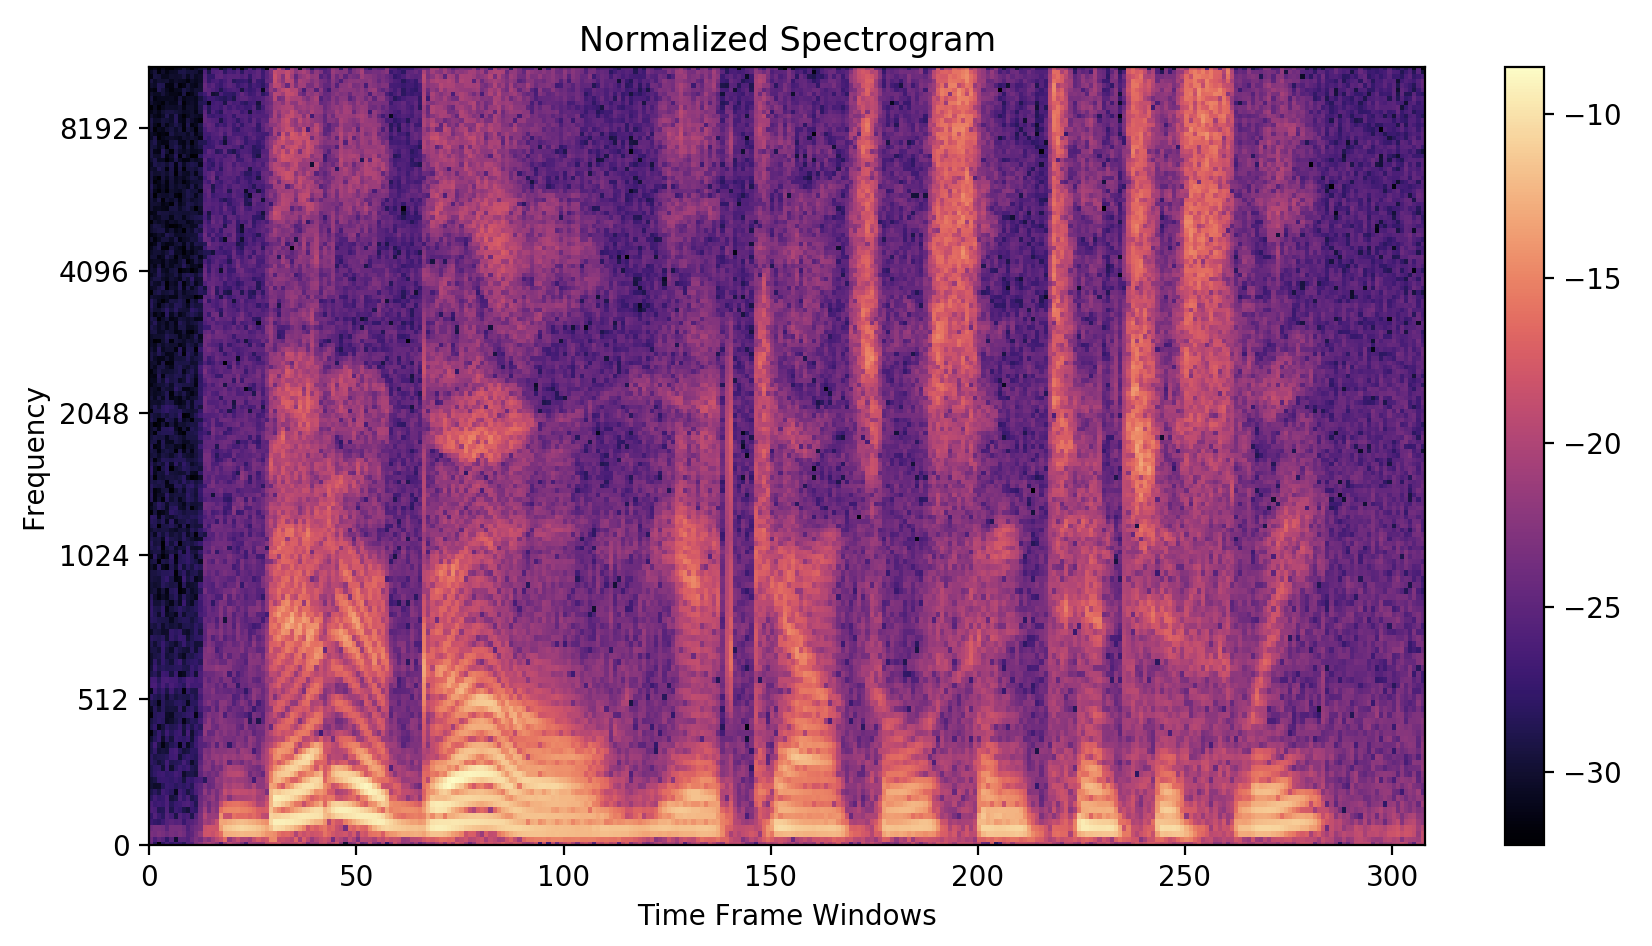
\includegraphics[width=\textwidth]{img/img_spectrogram.png}


%https://www.youtube.com/watch?v=UKHBWzoOKsY

\subsubsection{Mel Spectrum and Coefficients}
%https://en.wikipedia.org/wiki/Mel-frequency_cepstrum
%https://en.wikipedia.org/wiki/Mel_scale
%http://practicalcryptography.com/miscellaneous/machine-learning/guide-mel-frequency-cepstral-coefficients-mfccs/
%https://medium.com/analytics-vidhya/understanding-the-mel-spectrogram-fca2afa2ce53
%https://towardsdatascience.com/getting-to-know-the-mel-spectrogram-31bca3e2d9d0
%https://de.wikipedia.org/wiki/Mel_Frequency_Cepstral_Coefficients
%https://towardsdatascience.com/extract-features-of-music-75a3f9bc265d
%https://medium.com/analytics-vidhya/understanding-the-mel-spectrogram-fca2afa2ce53

A well-established finding from psychoacoustics is that human perception of sounds is not linear 
in frequency. Differences at lower frequencies are perceived as sounding `further apart' 
than the same absolute difference at higher frequencies. To reflect this, speech is mapped nonlinearly 
onto the mel scale
$$M(f) = 1125 \ln (1 + f/700)$$ 
typically using overlapping triangular windows whose spacing reflects human perception. 

To obtain the mel-frequency cepstrum, a number of additional operations are performed \citep{mel2012}.
At each of the mel frequencies, the log is taken of the power, which reflects the non-linear 
human perception of loudness.
Finally, the Discrete Cosine Transform of these values gives the mel-frequency cepstral coefficients, 
which together make up the mel frequency cepstrum.

%\subsubsection{}
%\subsubsection{}